% =====================================================================
%  SLAPBench  --  ECCV 2026 Workshop on Foundation and Generative
%  Models in Biometrics (FoundGen-Bio).  Official ECCV 2026 template.
%
%  BEFORE SUBMITTING, do the two TODOs marked below:
%    (1) put your OpenReview paper ID in the  ID=*****  option;
%    (2) for the camera-ready, switch the \usepackage lines as noted.
%  The `review' option anonymizes the author block automatically, so the
%  real names kept below never appear in the compiled review PDF.
% =====================================================================
\documentclass[runningheads]{llncs}

% TODO REVIEW: replace ***** with your OpenReview submission ID.
\usepackage[review,year=2026,ID=*****]{eccv}
% TODO FINAL (camera-ready): comment the line above and use the one below.
%\usepackage{eccv}

\usepackage{eccvabbrv}
\usepackage{graphicx}
\usepackage{amsmath,amssymb,amsfonts}
\usepackage{booktabs}
\usepackage{multirow}
\usepackage{colortbl}
\usepackage{xcolor}
\usepackage{float}
% axessibility ships with the official template and improves PDF
% accessibility. It compiles on Overleaf; keep it enabled there.
\usepackage[accsupp]{axessibility}
\usepackage[pagebackref,breaklinks,colorlinks,citecolor=eccvblue]{hyperref}

% ── Palette for the unified results table (AUC heatmap + collapse shading) ──
\definecolor{aucPerfect}{HTML}{3DBC6E}
\definecolor{aucStrong}{HTML}{8FCB7F}
\definecolor{aucMid}{HTML}{D7DC79}
\definecolor{aucWeak}{HTML}{F0A85C}
\definecolor{aucBad}{HTML}{E8736A}
\definecolor{collapseRed}{HTML}{F7D4D7}
\definecolor{funcGreen}{HTML}{D6EFD9}
\definecolor{grpBin}{HTML}{FBEFD9}
\definecolor{grpScore}{HTML}{E2ECFB}

\graphicspath{{figures/}}

\begin{document}

\title{SLAPBench: Benchmarking Multimodal Large Language Models
       for Four-Finger SLAP Fingerprint Verification}
\titlerunning{SLAPBench: MLLMs for Four-Finger SLAP Verification}

% Real author block (hidden automatically by the `review' option).
% TODO FINAL: add ORCIDs for the camera-ready version.
\author{Bibesh Pyakurel \and M.~G.~Sarwar Murshed}
\authorrunning{B.~Pyakurel and M.~G.~S.~Murshed}
\institute{Computer Science Department,
           University of Wisconsin--Green Bay, Green Bay, WI, USA}

\maketitle

\begin{abstract}
Four-finger SLAP (Slap Livescan Acquisition Protocol) fingerprint images
are the standard capture format at every US border entry
point~\cite{nist_sd302}, yet no benchmark exists to determine whether
multimodal large language models (MLLMs) can verify identity from them.
%
We introduce \textbf{SLAPBench}, the first benchmark for MLLM evaluation
on four-finger SLAP fingerprint verification, built on NIST Special
Database 302b (SD302b), an operational nail-to-nail dataset of 201
participants captured at 500 and 1000~PPI across multiple devices.
%
We construct 7,832 verification pairs under an impostor-heavy all-pairs
protocol (176~mated, 7,656~non-mated) and evaluate four open-source
models (InternVL3-8B-Instruct, Qwen2.5-VL-7B-Instruct,
Qwen3-VL-8B-Instruct, and Gemma-3-12B-IT) together with the proprietary
Claude Opus~4.8 under three prompting strategies: zero-shot, task
description, and a continuous similarity-scoring prompt.
%
Task-description prompting collapses all four open-source models to
near-100\% False Accept Rate~(FAR), and Gemma-3-12B collapses under
zero-shot as well. Claude Opus~4.8 alone resists collapse under both
prompts and attains the strongest binary result (FAR~$= 20.2\%$).
%
The similarity-scoring prompt eliminates collapse across the open-source
models and separates them by underlying capability. Claude Opus~4.8
reaches Area Under the ROC Curve (AUC)~$= 0.953$ with Equal Error
Rate~(EER)~$= 11.8\%$ and Gemma-3-12B reaches AUC~$= 0.837$
(EER~$= 15.1\%$), whereas InternVL3-8B produces inverted calibration
(AUC~$= 0.590$) and Qwen2.5-VL-7B yields near-random discrimination
(AUC~$= 0.567$).
%
Qwen3-VL-8B separates the two classes perfectly (AUC~$= 1.000$,
EER~$= 0.0\%$), which we report as a diagnostic rather than as evidence of
verification capability. Because SD302b supplies one SLAP capture per finger
position, mated pairs are cross-resolution, raising the concern that a model
could exploit resolution rather than identity. We run a matched-resolution
control that makes both classes cross-resolution, and the perfect separation
persists (AUC~$= 1.000$), which rules the resolution shortcut out. What
remains, and cannot be tested within SD302b, is that a mated pair is one
capture rendered twice, so the model may be detecting near-duplicate images
rather than identity. We therefore read the result as a cautionary finding
about how MLLM biometric benchmarks are assembled.
%
A stratified analysis across gender, race, and age finds that demographic
disparity tracks model \emph{weakness} rather than strength, inverting the
pattern reported for face benchmarks, though small subgroup sizes make
this an initial probe rather than a definitive audit.
Together these results establish the first SLAP-specific MLLM
verification baseline and show that prompt format governs whether
collapse occurs, while model architecture governs whether any
discriminative capability remains to be unlocked once collapse is removed.
\keywords{Fingerprint verification \and SLAP fingerprint \and Multimodal
large language models \and Biometric benchmark \and NIST SD302b \and
Similarity scoring \and Positive-bias collapse \and Protocol confound}
\end{abstract}

% ────────────────────────────────────────────────────────────────────────────
\section{Introduction}
\label{sec:intro}

Every US border entry point verifies traveler identity through a
\emph{SLAP} (Slap Livescan Acquisition Protocol) impression: four
fingers pressed simultaneously against a flat-bed scanner, matched
against the IDENT (DHS Automated Biometric Identification System)
database~\cite{nist_sd302}.
Unlike the rolled or plain single-finger impressions used in all prior
fingerprint MLLM benchmarks~\cite{fpbench2025}, SLAP images place four
overlapping fingers in a single frame, introduce ridge quality variation
across the capture, and require spatial reasoning about inter-finger
relationships.
SD302b sharpens the challenge further: collected at enrollment speed
during live border deployment, it is operational data, not a
competition set designed for controlled algorithmic evaluation.

Despite this operational importance, SLAP images have not been evaluated in
any multimodal LLM benchmark. The closest prior work, FPBench~\cite{fpbench2025},
evaluates 20~MLLMs on eight fingerprint tasks, but every task uses
\emph{individual} rolled or plain impressions from FVC datasets and NIST
SD302d/SD301a, so none exercises the inter-finger spatial reasoning SLAP
images require.

A second question concerns how prompting affects collapse. Face and
fingerprint benchmarks have documented \emph{positive-bias collapse}, where a
model answers ``same person'' regardless of input and so scores 50\% on a
balanced set while appearing to function~\cite{facerecbench2025,fpbench2025}.
Binary forced choice is the format used in every prior biometric MLLM
benchmark; whether it collapses on SLAP data, and whether other prompt designs
prevent it, bears on a failure mode no border application could tolerate,
namely a system that accepts every traveler.
We stress that SLAPBench is an \emph{evaluation probe} of current MLLM
behavior on SLAP-format images, not a proposed deployment system. Our aim
is to characterize how these models succeed and fail under different
prompts, not to advocate their use in operational border verification.

This paper makes the following contributions:

\begin{enumerate}
  \item \textbf{SLAPBench}, the first benchmark for MLLM evaluation on
        four-finger SLAP fingerprint verification, built on NIST SD302b, an
        operational dataset that no prior fingerprint MLLM work has used.

  \item \textbf{A reproducible evaluation protocol} of 7,832~fixed pairs
        (176~mated, formed across resolution because SD302b provides a
        single SLAP capture per finger position; 7,656~non-mated, covering
        all $\binom{88}{2}$ subject combinations per FRGP), released as a
        fixed pair manifest with demographic metadata that supports a
        stratified analysis across gender, race, and age.

  \item \textbf{Systematic evidence of positive-bias collapse on SLAP data.}
        Five of ten binary prompting configurations collapse to accepting
        nearly every pair as genuine. All four open-source models collapse
        under task-description prompting and Gemma-3-12B collapses under
        zero-shot as well, while the proprietary Claude Opus~4.8 resists
        collapse under both prompts. Collapse is therefore largely a
        property of the prompt format, but a sufficiently capable model can
        overcome it.

  \item \textbf{A similarity-scoring prompt that exposes model capability.}
        Scoring eliminates collapse in all four open-source models, yet
        discrimination still ranges from functional (Claude Opus~4.8,
        Gemma-3-12B) to near-random or inverted (Qwen2.5-VL-7B,
        InternVL3-8B). Scoring is thus necessary but not sufficient, and
        model architecture sets the ceiling
        (Table~\ref{tab:main_results}).

  \item \textbf{A cautionary analysis of a perfect benchmark score.}
        Qwen3-VL-8B attains AUC~$= 1.000$ under scoring. A matched-resolution
        control that removes resolution as a class cue leaves the perfect
        separation intact, which excludes the resolution shortcut; the
        single-capture design of SD302b nonetheless leaves near-duplicate
        detection in place, and no configuration of the dataset can separate
        it from identity matching. We offer this as evidence that near-perfect
        MLLM biometric results warrant a protocol audit before they are read
        as capability.

  \item \textbf{Public release} of the evaluation code, the fixed pair
        manifest, the raw result CSVs, and the per-pair score files, so that
        every number reported here can be recomputed. The repository link is
        withheld for double-blind review and will be included in the
        camera-ready version.
\end{enumerate}

% ────────────────────────────────────────────────────────────────────────────
\section{Related Work}
\label{sec:related}

\textbf{Fingerprint recognition.}
Classical pipelines of acquisition, enhancement, feature extraction, and
matching~\cite{maltoni_handbook} have been advanced at each stage by deep
learning: FingerNet unifies ridge-orientation and minutiae
extraction~\cite{fingerNet}, DeepPrint learns fixed-length embeddings for
scalable verification~\cite{deepprint}, and commercial matchers such as
VeriFinger~\cite{verifinger} provide operational FAR/FRR baselines. All solve
recognition with dedicated learned representations, unlike the zero-shot
reasoning an MLLM performs. SLAP segmentation is studied
separately~\cite{murshed2024SlapSeg}; to our knowledge no prior work
evaluates end-to-end MLLM performance on SLAP images.

\textbf{MLLM biometric benchmarks.}
FaceXBench~\cite{facexbench2024} evaluates 28~models on 5{,}000 face-task
questions and finds chain-of-thought prompting consistently \emph{degrades}
performance, a caution against assuming more context helps.
FaceRecBench~\cite{facerecbench2025} benchmarks 27~MLLMs on face verification
and reports two findings we revisit for fingerprints: many models collapse to
50\% accuracy by always accepting or rejecting, and the best model carries the
strongest demographic bias; a follow-up extends this to heterogeneous face
recognition with similar capability gaps~\cite{shahreza2026hfr}.
FPBench~\cite{fpbench2025} is closest to us, evaluating 20~MLLMs on eight
single-finger fingerprint tasks under MCQ prompting. We differ in three ways:
four-finger SLAP images requiring spatial reasoning; continuous similarity
scoring alongside binary classification; and the operational SD302b dataset.
Across these benchmarks, response collapse recurs and has been attributed to
training-data priors favouring ``same'' together with the ambiguity of
biometric comparison in language; we give the first quantitative account on
SLAP images and show that continuous scoring removes it.

% ────────────────────────────────────────────────────────────────────────────
\section{Dataset and Data Preparation}
\label{sec:dataset}

\subsection{NIST Special Database 302b}

NIST SD302b~\cite{nist_sd302} is a subset of the Nail-to-Nail (N2N)
Fingerprint Challenge dataset collected by the Intelligence Advanced
Research Projects Activity (IARPA).
The database contains fingerprint images from 201~participants captured
using multiple devices at two resolutions: 500~PPI (standard operational
resolution) and 1000~PPI (high resolution for research).
Participants span diverse demographics including age (range: 18--70),
gender, race, and occupational background (work type), enabling
stratified fairness analysis.
We focus exclusively on \textbf{FRGP 13} (right four-finger SLAP) and
\textbf{FRGP 14} (left four-finger SLAP) images captured by
\textbf{Device~R}.
Device~R images in SD302b are captured natively at 1000~PPI, and the
corresponding 500~PPI versions are supplied for compatibility with
500~PPI fingerprint algorithms. The 500~PPI image is therefore a
downsampled version of the same capture rather than a second, independent
impression.
We confirmed this directly against the distributed file structure rather
than relying on the documentation alone. Across the 88~clean subjects, the
Device~R SLAP set contains exactly 352~files, one per
(subject,~FRGP,~resolution) triple, and every file name has the form
\texttt{SUBJECT\_R\_\{500\textbar1000\}\_slap\_\{13\textbar14\}.png} with
no impression or sequence index. Each (subject,~FRGP) combination is
therefore represented by exactly one capture, available at two resolutions,
and SD302b offers no repeat SLAP impression for any subject and finger
position.
This is a property of the database rather than a choice on our part, and it
fixes the form a mated pair can take: each mated pair is a
\emph{same-capture cross-resolution} comparison between the native
1000~PPI image and its 500~PPI counterpart, not a comparison of two
independent impressions.
Sections~\ref{sec:pairs} and~\ref{sec:discussion} set out what this
structure does and does not permit us to conclude.

\textbf{Data preparation.}
Following the SD302b documentation we exclude errata-flagged subjects
(labeling errors), roll images (devices U, V), FRGP~15 thumb-slaps, and
pre-cropped segmented crops, and keep only subjects with both R-500 and R-1000
captures. Of the \textbf{201} participants, \textbf{92} have Device~R
four-finger SLAP at both FRGP~13/14 and both resolutions; removing
errata/incomplete subjects leaves \textbf{88} clean subjects. The verification
experiment therefore uses \textbf{352 Device~R images}
(88~subjects $\times$ 2~FRGP $\times$ 2~resolutions).
These are a subset of a broader curated active set of \textbf{584 SLAP
images}, which additionally retains Device~S 500~PPI captures and the
excluded subjects' images for future SLAP tasks; only the 352 Device~R
images above enter the pair construction of this paper.
For each image, we build a master dataframe recording image-level
metadata (device, resolution, FRGP, dimensions, integrity checksum),
per-finger segmentation ground truth (bounding-box coordinates and
rotation angle $\theta$ from the SD302b segmentation CSVs), and
participant demographics.

\textbf{Ground-truth segmentation.}
SD302b ships per-image segmentation CSVs giving bounding-box coordinates and a
rotation angle for each finger (dedicated SLAP segmentation systems address the
same step~\cite{murshed2024SlapSeg}); a representative overlaid image appears in
the supplementary material (Fig.~S1). For verification we use the full SLAP
images without cropping, as operational pipelines do. Because a single frame
holds four overlapping fingers of similar morphology, any two SLAP images look
globally alike whether mated or not, which underlies the positive-bias collapse
analyzed in Section~\ref{sec:discussion}.

% ────────────────────────────────────────────────────────────────────────────
\section{Evaluation Protocol and Methodology}
\label{sec:method}

\subsection{Pair Construction}
\label{sec:pairs}

We construct mated and non-mated verification pairs following the
all-pairs protocol used in FaceRecBench~\cite{facerecbench2025} and
FPBench~\cite{fpbench2025}.

\textbf{Mated (genuine) pairs.}
For each FRGP $\in \{13, 14\}$, we pair each subject's native 1000~PPI
image with the corresponding downsampled 500~PPI version of the
\emph{same capture}.
With 88~clean subjects, this yields 88~mated pairs per FRGP and 176~mated
pairs in total.
Each eligible subject contributes exactly one such comparison per SLAP
position, so the count of mated comparisons is fixed at 176 by the
structure of the database rather than by a sampling decision.

\textbf{Non-mated (impostor) pairs.}
For each FRGP, we form all pairings of distinct subjects.
With 88 subjects, this yields $\binom{88}{2} = 3{,}828$ unique non-mated
pairs per FRGP, and $3{,}828 \times 2 = 7{,}656$ non-mated pairs in total.
We verify that no non-mated pair involves the same subject.
This exhaustive construction follows standard practice in biometric
benchmarking~\cite{facerecbench2025} and provides more reliable
error-rate estimates than random subsampling.

The resulting \textbf{7,832~pairs} (176~mated $+$ 7,656~non-mated), released as
a fixed manifest, form an intentionally impostor-heavy all-pairs protocol, not
a balanced set: non-mated trials grow combinatorially with subjects while mated
trials are capped by samples per subject. This imbalance is standard in
biometrics, so we emphasize FAR, FRR, AUC, EER, and TAR at low FAR rather than
overall accuracy, which the non-mated majority dominates.

\textbf{Resolution structure and its consequence.}
Mated pairs are cross-resolution (1000~PPI vs.\ 500~PPI), whereas
non-mated pairs are drawn from the 500~PPI pool and are therefore
same-resolution (500~PPI vs.\ 500~PPI).
The two classes consequently differ in a property that has nothing to do
with identity, and a model could in principle separate them by reading
resolution or appearance statistics instead of comparing ridge structure.
We state this plainly at the outset because it governs how the strongest
results in Section~\ref{sec:results} may be read. To settle it we also build a
matched-resolution variant in which the non-mated pairs are formed as
1000~PPI vs.\ 500~PPI, so both classes share the same resolution structure;
Section~\ref{sec:perfect} reports that the strongest result is unchanged under
this control, so the ranking is not an artefact of resolution mismatch.
The collapse results are not affected either, for the
reason given in Section~\ref{sec:limitations}: FAR is computed on non-mated
pairs, which are same-resolution by construction and involve no
cross-resolution comparison at all.
Each pair record also carries demographic metadata (age, gender, and race
of both subjects), which supports the stratified analysis in
Section~\ref{sec:fairness}.

\subsection{Models}

We evaluate four open-source MLLMs and one proprietary frontier model,
selected for their demonstrated performance on fingerprint and face
biometric benchmarks and to span a range of model scales and access
modes (locally hosted open weights versus a commercial API):

The four open-source models span the systems that lead recent fingerprint and
face benchmarks: \textbf{InternVL3-8B-Instruct}~\cite{internvl3} (bfloat16,
$\sim$16~GB), a top open-source performer in FPBench;
\textbf{Qwen2.5-VL-7B-Instruct}~\cite{qwen25vl}, the architecture strongest in
FaceRecBench; its successor \textbf{Qwen3-VL-8B-Instruct}~\cite{qwen3vl}; and
\textbf{Gemma-3-12B-IT}~\cite{gemma3}, the largest local model. The latter
three use 4-bit NF4 quantization ($\sim$6--8~GB). We add
\textbf{Claude Opus~4.8}~\cite{claudeopus} (Anthropic API, undisclosed weights)
as a high-capability proprietary reference. Exact identifiers are
\texttt{InternVL3-8B-Instruct}, \texttt{Qwen2.5-VL-7B-Instruct},
\texttt{Qwen3-VL-8B-Instruct}, \texttt{Gemma-3-12B-IT}, and
\texttt{claude-opus-4-8}; all runs were collected in June~2026.

The open-source models run via HuggingFace \texttt{transformers} on a single
NVIDIA RTX~4080~SUPER (16.9~GB) with deterministic decoding
(\texttt{temperature}$=0$); Claude is queried as independent stateless
requests. The two images and the text prompt are the only inputs to any
model: no filenames, subject IDs, resolution labels, or demographics appear in
a request, so no model has access to ground-truth identity at inference.

\subsection{Prompting Strategies}
\label{sec:prompts}

We evaluate three prompting strategies, using a fixed system prompt
``\textit{You are an expert fingerprint examiner.}'' across all settings.
Before inference, every image is converted to grayscale, contrast-normalized
(autocontrast), and resized to $448\times448$ pixels, identically for all
five models; this common preprocessing also equalizes the pixel dimensions
of the 500 and 1000~PPI images, though it does not remove the underlying
near-duplicate relationship between a mated pair
(Section~\ref{sec:discussion}).
Under \textbf{zero-shot} the model receives the two images and the binary
question ``Do these two images belong to the same person? (A) Yes (B) No.''
\textbf{Task description} prepends a sentence explaining that repeated captures
of one finger vary slightly while ridge patterns persist, before the same
binary question. \textbf{Similarity scoring} instead asks for a single integer
from 0 (certainly different) to 100 (certainly the same). The three templates
are reproduced verbatim in the supplementary material (Fig.~S4).

\textbf{Zero-shot (ZS).}
The model receives the two SLAP images and a minimal binary question:
\textit{``Do these two images belong to the same person?''} with
options (A) Yes and (B) No.
This is the standard protocol in FPBench and
FaceRecBench~\cite{fpbench2025,facerecbench2025}, enabling direct
comparison.

\textbf{Task description (TD).}
The prompt additionally explains the nature of SLAP images and the
effect of repeated captures (pressure variation, slight movement)
before posing the same binary question.
This tests whether domain context reduces the collapse tendency.

\textbf{Similarity scoring (SS).}
Rather than a binary choice, the model is asked to return a single
integer between 0 and 100 representing its confidence that the two
images belong to the same person: 0 means completely certain they are
different people; 100 means completely certain they are the same person.
The model is instructed to reply with the number only, with no
explanation or label.
This framing treats the model's output as a direct confidence
percentage, avoiding the need to cross a forced binary decision boundary.

\subsection{Response Parsing and Metrics}

For binary prompts we parse responses with the three-step fallback of
VLMEvalKit~\cite{vlmevalkit} (leading A/B; then A/B anywhere; then keyword
matching on SAME/YES/GENUINE vs.\ DIFFERENT/NO/IMPOSTOR), marking anything
unmatched INVALID. For the scoring prompt we take the first integer via regex
and clamp it to $[0,100]$.
We report standard verification metrics: for binary prompts, accuracy, FAR,
FRR, and collapse detection (any answer chosen $>$95\% of the time); for
scoring, mean confidence on mated and non-mated pairs, their separation
$\Delta$, EER, and AUC from a threshold sweep over $[0,100]$.

% ────────────────────────────────────────────────────────────────────────────
\section{Results}
\label{sec:results}

\subsection{Binary Prompting: Collapse Under Task Description}

\textbf{Positive-bias collapse} appears in five of ten binary
configurations, with FAR reaching 96.4--100\%
(Table~\ref{tab:main_results}). All four open-source models collapse under
the task-description prompt, and Gemma-3-12B collapses under zero-shot as
well. The proprietary Claude Opus~4.8 is the sole exception, resisting
collapse under both prompts.

% ── Unified results table (binary + similarity scoring) ─────────────────────
\begin{table}[t]
\centering
\caption{SLAPBench verification results on NIST SD302b (7,832 pairs:
  176~genuine $+$ 7,656~impostor). Models are ordered by similarity-scoring
  AUC. \textbf{Binary prompting} reports accuracy and FAR for zero-shot~(ZS)
  and task-description~(TD); red cells mark collapsed configurations
  (FAR~$\geq$95\%, the model answers ``same person'' on nearly every pair),
  the green cell marks the single strongest binary configuration.
  \textbf{Similarity scoring} reports mean confidence on genuine~(Gen) and
  impostor~(Imp) pairs, separation~$\Delta$, EER, AUC (shaded green$\rightarrow$red
  for strong$\rightarrow$random discrimination), and TAR at FAR~$=0.1\%$.
  Low binary accuracy in collapsed runs ($\approx$2--6\%) reflects the
  43:1 impostor-to-genuine imbalance; FAR, AUC, and EER are the meaningful
  measures. Claude Opus~4.8 is the only model that resists collapse under
  \emph{both} prompts and attains the strongest binary configuration
  (ZS FAR 20.2\%).}
\label{tab:main_results}
\renewcommand{\arraystretch}{1.25}
\setlength{\tabcolsep}{4.5pt}
\footnotesize
\begin{tabular}{c l cccc cccccc}
\toprule
& & \multicolumn{4}{c}{\cellcolor{grpBin}\textbf{Binary Prompting}}
  & \multicolumn{6}{c}{\cellcolor{grpScore}\textbf{Similarity Scoring (0--100)}} \\
\cmidrule(lr){3-6}\cmidrule(lr){7-12}
\textbf{\#} & \textbf{Model}
  & \textbf{ZS Acc} & \textbf{ZS FAR} & \textbf{TD Acc} & \textbf{TD FAR}
  & \textbf{Gen} & \textbf{Imp} & \boldmath{$\Delta$} & \textbf{EER}
  & \textbf{AUC} & \textbf{TAR\textsubscript{0.1\%}} \\
\midrule
1 & Qwen3-VL-8B
  & 74.1\% & 26.5\% & 3.3\% & \cellcolor{collapseRed}98.9\%
  & \textbf{100.0} & 63.8 & $+$36.2 & \textbf{0.00\%}
  & \cellcolor{aucPerfect}\textbf{1.000} & \textbf{100.0\%} \\
2 & Claude Opus 4.8
  & \textbf{80.3\%} & \cellcolor{funcGreen}\textbf{20.2\%} & 50.2\% & 50.9\%
  & 91.3 & 48.4 & $+$42.9 & 11.75\%
  & \cellcolor{aucStrong}0.953 & 56.8\% \\
3 & Gemma-3-12B
  & 5.7\% & \cellcolor{collapseRed}96.4\% & 2.3\% & \cellcolor{collapseRed}100.0\%
  & 75.8 & 63.3 & $+$12.5 & 15.10\%
  & \cellcolor{aucMid}0.837 & 23.3\% \\
4 & InternVL3-8B
  & 29.3\% & 72.3\% & 2.2\% & \cellcolor{collapseRed}100.0\%
  & 57.7 & 79.1 & $-$21.4 & 48.09\%
  & \cellcolor{aucWeak}0.590 & 0.0\% \\
5 & Qwen2.5-VL-7B
  & 32.0\% & 69.6\% & 2.2\% & \cellcolor{collapseRed}100.0\%
  & 95.0 & 90.1 & $+$4.9 & 43.34\%
  & \cellcolor{aucBad}0.567 & 0.0\% \\
\bottomrule
\end{tabular}
\end{table}

All five collapsed runs land at roughly 2.2--5.7\% overall accuracy rather
than the 50\% that a balanced set would produce, because accepting all
7,832 pairs classifies only the 176 mated pairs correctly (2.25\% of the
total) and accepts all 7,656 impostors.
FAR is the meaningful measure here, and at 96.4--100\% it describes a
complete verification failure.

Under zero-shot prompting, four models avoid collapse (FAR 20.2--72.3\%,
Table~\ref{tab:main_results}). \textbf{Claude Opus~4.8 gives the strongest
binary result overall} (80.3\% accuracy, FAR 20.2\%), ahead of the best
open-source model, Qwen3-VL-8B (74.1\%, FAR 26.5\%); InternVL3-8B and
Qwen2.5-VL-7B trail at FAR 72.3\% and 69.6\%. Gemma-3-12B is the exception,
collapsing even under zero-shot (FAR 96.4\%). Across these non-collapsed
runs nearly every mated pair is accepted (FRR~$\leq$0.6\%), so ``different''
answers fall almost exclusively on impostor pairs.

Adding domain context (TD) collapses all four open-source models to
near-100\% FAR, including Qwen3-VL-8B which had the best open-source ZS
result. \textbf{Claude Opus~4.8 is the lone exception}: under TD it remains
balanced (50.2\% accuracy, FAR 50.9\%, answering ``same person'' on only
52\% of pairs), neither collapsing nor degrading to the open-source
failure mode.
For the open-source models, prompting complexity increases the false
accept rate rather than reducing it, confirming the FaceXBench and FPBench
observation that additional context does not help and actively hurts in
biometric binary tasks~\cite{facexbench2024,fpbench2025}.
That Claude Opus~4.8 alone withstands this effect suggests the collapse is
not an inevitable property of binary prompting but one that sufficiently
capable models can resist.

\subsection{Similarity Scoring: Discriminative Signal Revealed}

The similarity-scoring prompt eliminates collapse across all four
open-source models: no model produces a single constant output, and mated
and non-mated pairs occupy distinguishable (though not always separable)
score ranges. Figure~\ref{fig:score_dist} shows the distributions for all
five models, and the scoring block of Table~\ref{tab:main_results} gives the
metrics.

\begin{figure}[tbp]
  \centering
  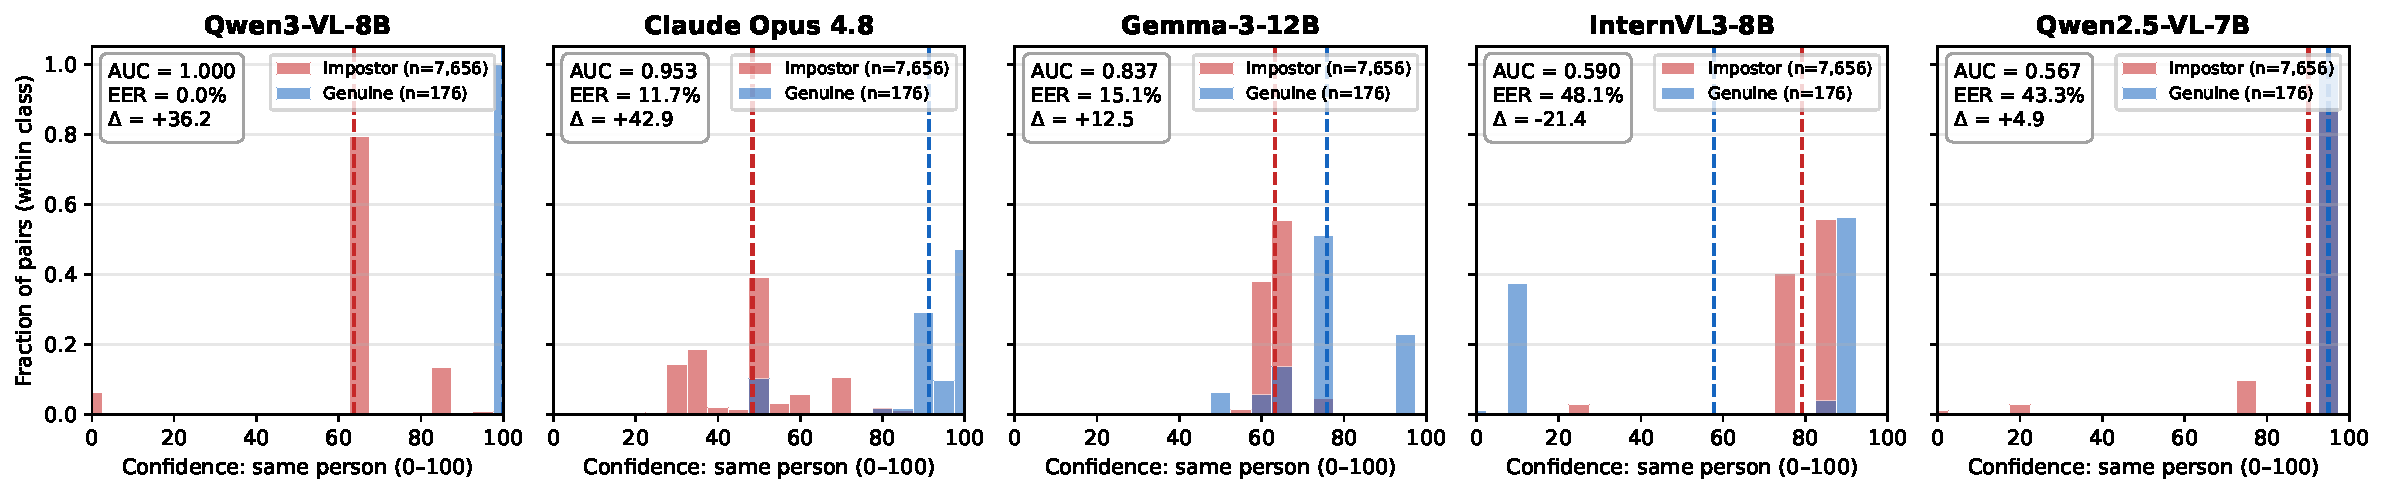
\includegraphics[width=0.82\linewidth]{fig_score_dist_all.pdf}
  \caption{Score distributions under the similarity-scoring prompt
    (7,832 pairs). Bars give the fraction of pairs \emph{within each class},
    normalized separately to offset the 176:7{,}656 mated-to-non-mated
    imbalance; dashed lines mark per-class means; each panel is annotated with
    AUC, EER and mean separation $\Delta$. Scores are discrete, so no
    continuous density is fitted. The first three models discriminate;
    InternVL3-8B is inverted ($\Delta = -21.4$, with a bimodal mated
    distribution) and Qwen2.5-VL-7B is compressed, piling both classes
    near 95.}
  \label{fig:score_dist}
\end{figure}

The models split into two tiers (Table~\ref{tab:main_results}).
\textbf{Qwen3-VL-8B} separates the classes completely (AUC~$= 1.000$,
EER~$= 0.0\%$); a result this clean calls for scrutiny rather than
celebration, and we examine it in Section~\ref{sec:perfect}.
\textbf{Claude Opus~4.8} is the strongest graded discriminator
(AUC~$= 0.953$), with the widest mated-to-non-mated gap of any model
($+$42.9~points), and \textbf{Gemma-3-12B} is functional but weaker
(AUC~$= 0.837$).
The other two fail in opposite ways: \textbf{InternVL3-8B} is
\emph{inverted}, reporting higher confidence on impostors than on genuine
matches ($\Delta = -21.4$, AUC~$= 0.590$), while \textbf{Qwen2.5-VL-7B} is
\emph{compressed}, over 90\% confident on nearly every pair regardless of
identity ($\Delta = +4.9$, AUC~$= 0.567$). Both are near chance and neither
admits a threshold that accepts a mated pair before an impostor, so both
reach TAR~$= 0.0\%$ at FAR~$= 0.1\%$. Per-hand behaviour is symmetric for
every model, so we omit the FRGP~13/14 split.

Scoring therefore eliminates collapse in all four open-source models without
guaranteeing meaningful discrimination: Qwen3-VL-8B, Claude, and Gemma
separate the classes, whereas InternVL3-8B and Qwen2.5-VL-7B stay effectively
random. Once collapse is removed it is this architectural split, not the
prompt, that separates success from failure.
\textbf{The binary collapse in Table~\ref{tab:main_results} is thus a
prompt-format artifact; whether discriminative capability can be
unlocked by scoring depends on model architecture.}
The supplementary material (Fig.~S2) grounds these aggregate numbers in two
real pairs: on a mated pair every model but InternVL3-8B reports high
confidence, while InternVL3 returns~9; on a non-mated pair Qwen3-VL-8B,
Claude, and Gemma assign lower confidence than InternVL3-8B~(85) and
Qwen2.5-VL-7B~(95), which falsely accept it.

Figure~\ref{fig:roc} plots the full ROC curves for the four open-source
models and Claude Opus~4.8.
The inset shows the low-FAR operating region (FAR $\leq 0.05$),
where Qwen3-VL-8B achieves TAR~$= 100\%$ even at FAR~$= 0.1\%$.
The TAR\textsubscript{0.1\%} column of Table~\ref{tab:main_results}
reports TAR at FAR~$= 0.1\%$, the standard operational stringency target in
border biometrics. InternVL3-8B and Qwen2.5-VL-7B reach 0\% here because
their score distributions offer no threshold that holds FAR below 0.1\%
while still accepting any mated pair, a direct consequence of inverted
calibration (InternVL3) and compressed scoring (Qwen2.5).

\begin{figure}[tbp]
  \centering
  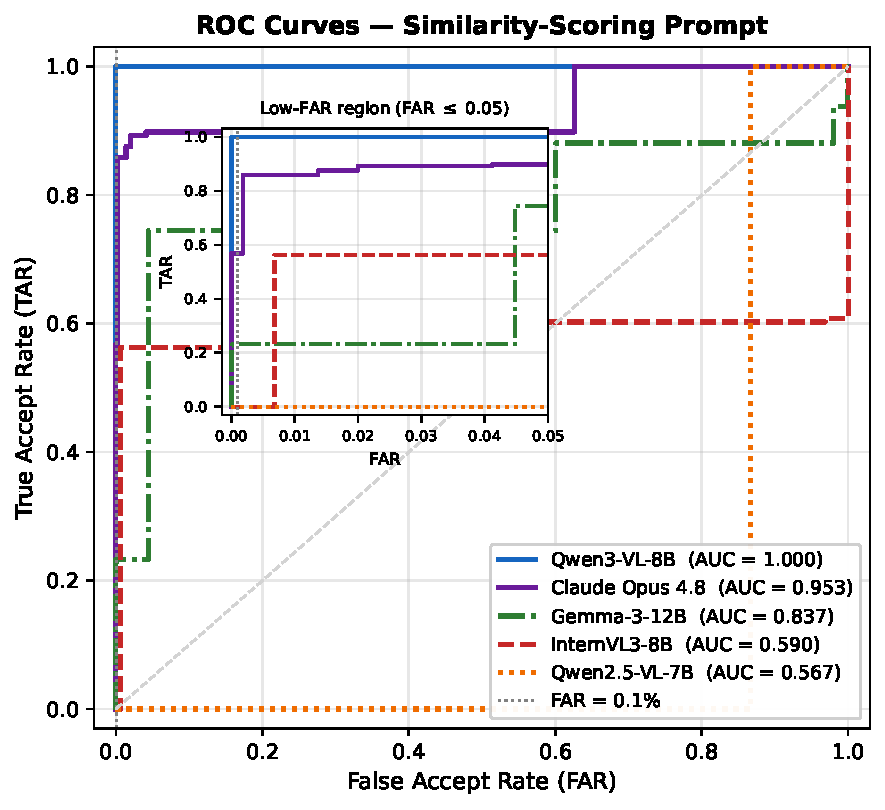
\includegraphics[width=0.48\linewidth]{fig_roc_curves.pdf}
  \caption{ROC curves under the similarity-scoring prompt (7,832 pairs)
    for the four open-source models and the proprietary Claude Opus~4.8.
    The inset magnifies the low-FAR region (FAR $\leq 0.05$). The dotted
    vertical line marks FAR~$= 0.1\%$.
    Qwen3-VL-8B (AUC~$= 1.000$) achieves perfect discrimination, Claude
    Opus~4.8 (AUC~$= 0.953$) and Gemma-3-12B (AUC~$= 0.837$) are clearly
    functional, while InternVL3-8B and Qwen2.5-VL-7B perform near random
    (AUC~$= 0.590$ and $0.567$).}
  \label{fig:roc}
\end{figure}

\subsection{Demographic Fairness}
\label{sec:fairness}

FaceRecBench reports that the best face-verification MLLM also carries the
strongest demographic bias~\cite{facerecbench2025}; we test the pattern on
SLAP by recomputing similarity-scoring performance within gender, race, and
age subgroups for the three discriminating models (full protocol, per-subgroup
table, and plot in the supplementary material). The pattern runs
\emph{opposite} to FaceRecBench's: on SLAP data the stronger models look
fairer. Claude Opus~4.8 varies by at most 1.5~AUC points across gender, whereas
the weakest discriminator, Gemma-3-12B, shows the widest spread; Qwen3-VL-8B is
uniformly perfect, equally consistent with a group-invariant representation and
with the non-identity shortcut of Section~\ref{sec:perfect}. To the extent the
small subgroups support any reading, disparity tracks model \emph{weakness}
rather than strength. We treat this as an initial, hypothesis-generating probe
on a single database rather than an audit.

\subsection{Relationship to Prior Work}

We do not compare numbers directly with FPBench~\cite{fpbench2025}: it uses
individual rolled and plain impressions under a four-option MCQ format,
whereas SLAPBench uses four-finger captures under binary or continuous
scoring, so the datasets, image types, and metrics are not comparable. What
both establish, and ours confirms, is the qualitative pattern that binary
prompting on fingerprints collapses open-source models regardless of image
type. The two benchmarks are complementary rather than competing.

% ────────────────────────────────────────────────────────────────────────────
\section{Discussion}
\label{sec:discussion}

\subsection{Why Binary Prompts Collapse on SLAP Data}

Collapse follows a consistent signature: every collapsed run has FRR~$= 0\%$
and FAR~$\geq 96.4\%$, the mark of a model whose prior for ``same person'' is
so strong that no visual evidence moves it toward ``B.'' Two structural
factors make this prior stronger for SLAP than for the single-finger images
of FPBench. First, any two SLAP images share the same gross morphology (four
fingers, similar spacing, skin texture, and orientation), so their global
similarity is far higher than between two isolated rolled impressions,
whether the pair is mated or not; the surface-level similarity prior is thus
satisfied for every pair regardless of identity. Second, the task-description
prompt, which states that ``the same person's fingers produce slightly
different images each time,'' \emph{increases} collapse: it primes a schema in
which variation is a property of mated pairs and lowers the ``same'' threshold
across all inputs, the model having read ``same person'' twice before seeing
either image. The lesson for benchmark design is that naturalistic domain
descriptions can worsen collapse by legitimizing visual differences.

This also explains the exception. Claude Opus~4.8 resists collapse under both
prompts exactly as the mechanism predicts, rejecting about half of impostors
even under task description (FAR 50.9\%) and four-fifths under zero-shot
(FAR 20.2\%). A model with identity evidence strong enough to overcome the
similarity prior is not forced into the degenerate ``same'' response. Collapse
is therefore a capability threshold, not a fixed property of the binary
format: the same format that collapses four open-source models leaves the
strongest one balanced.

\subsection{Why Similarity Scoring Breaks Collapse}

The scoring prompt resolves the same underlying problem by changing what
the model is asked to optimize.
Under binary prompting, the model must commit to a categorical label
against its own prior; the prior wins.
Under scoring, the model places a continuous estimate on a calibrated
scale, a task that requires reporting a degree of confidence rather than
crossing a decision boundary.
This framing lets the model's uncertainty about impostor pairs surface as a
lower score instead of being suppressed into the same ``A'' response it
gives to mated pairs.

The scoring prompt eliminates collapse in all four open-source models, but
the resulting distributions show that scoring is necessary without being
sufficient. It reveals whether discriminative capability exists; it does
not confer it. The two models that lack it are InternVL3-8B and
Qwen2.5-VL-7B (Fig.~\ref{fig:score_dist}, rightmost panels).

The two failures differ in kind. \textbf{InternVL3-8B} is \emph{inverted},
scoring impostors above genuine pairs; we suspect its encoder keys on
fine-grained ridge texture, which contrasts more strongly across two
different subjects than between two renderings of one capture, so scoring
faithfully reports this signal in the wrong direction. \textbf{Qwen2.5-VL-7B}
is instead \emph{compressed}: correctly ordered but confined to a narrow
high-confidence band, the scoring-domain echo of the same similarity prior
that drives its binary collapse. In neither case can scoring manufacture
discrimination the representation does not encode.

Why does scoring unlock the stronger models but not these? The most
actionable explanation is that its calibrated anchors tell the model
\emph{where to look} (ridge flow, minutiae) and \emph{what to report}
(a value on a fixed scale) rather than forcing a binary commit, and only
models with sufficient visual reasoning (Qwen3, Claude) can act on them.
Recency of instruction-tuning on similarity/scoring tasks may compound this.
The practical implication is that \textbf{a calibrated scoring prompt is a
more effective probe of MLLM biometric capability than binary forced choice,
but only when the architecture can exploit it.}

\subsection{A Perfect Score Is a Diagnostic, Not a Capability Claim}
\label{sec:perfect}

Qwen3-VL-8B attains AUC~$= 1.000$ with EER~$= 0.0\%$. We do not present
this as a capability result, and we argue that it should not be read as
one. Our position is that the number is explained by the structure of the
protocol rather than by the model's verification ability, and this
subsection sets out the evidence for that conclusion. We treat the episode
as the most useful finding in the paper for benchmark designers, because it
shows how readily a SLAP verification protocol can manufacture a perfect
score.

The behavior underlying the number is narrow and revealing. Qwen3-VL-8B
assigns a score of \emph{exactly} 100 to all 176 mated pairs: the mated
score distribution has a single distinct value. Its non-mated scores, by
contrast, take only seven distinct values
($\{0, 30, 45, 65, 85, 90, 95\}$, mean 63.8), and \emph{no} non-mated pair
is ever scored above 95. Perfect separation is therefore not the product of a finely graded similarity
judgment; it follows from a coarsely quantized output in which a single
response, 100, is reserved for the mated class and never emitted otherwise.
Any mechanism that saturates the mated class in this way reproduces
AUC~$= 1.000$ exactly, whether or not it compares ridge structure, and a model
doing genuine forensic comparison would be expected to show at least some
graded uncertainty across 176 subjects. By contrast Claude Opus~4.8, which is
graded, uses nine distinct mated and 48 distinct non-mated values on the same
pairs.

The \textbf{resolution shortcut} is the explanation that fits this signature
most economically, and it is the one we set out to test. In the main protocol
mated pairs are cross-resolution (1000 vs.\ 500~PPI) while non-mated pairs are
same-resolution (500 vs.\ 500), so a model that merely detects a resolution or
downsampling difference could separate the classes without comparing identity.

We therefore ran the \textbf{matched-resolution control} of
Section~\ref{sec:pairs}, rebuilding every non-mated pair as subject~A at
1000~PPI versus subject~B at 500~PPI so that both classes share an identical
1000-to-500 structure and differ only in identity. We evaluated the complete
right-hand benchmark under this control (FRGP~13: 88 mated and all 3{,}828
non-mated pairs). The result is essentially unchanged: Qwen3-VL-8B again scores
exactly 100 on every mated pair, again never scores a non-mated pair above 95,
and again attains AUC~$= 1.000$ with EER~$= 0.0\%$, the non-mated mean moving
only from 65.6 to 65.3. Making resolution non-diagnostic had no measurable
effect, so \textbf{the resolution shortcut does not explain the result and we
exclude it}.

What the control cannot remove is \textbf{near-duplicate detection}, which now
becomes the leading account. A mated pair is one capture rendered at two
scales, so the two images are near-duplicates at the signal level, with far
stronger low-level correspondence than a deployed matcher sees between two
independent impressions; a non-mated pair joins two different captures under
the control just as in the main protocol. A model asking ``are these two
renderings of one image?'' rather than ``are these two impressions of one
finger?'' would produce exactly this behaviour, and rearranging resolutions
cannot disturb it. Critically, SD302b cannot adjudicate this: Device~R holds
one capture per subject and finger, and the Device~R and Device~S subject
pools are disjoint, so no mated pair in the database can be formed from two
independent impressions. The question is unanswerable within this dataset and
needs a database with repeat SLAP captures.

\textbf{Memorization} we set aside. SD302b is public, so contamination cannot
be excluded outright, but had the model memorized identity labels that
knowledge should transfer across prompts; instead its zero-shot binary FAR is
26.5\% and it collapses under task description. Nor would memorization explain
why no other model reproduces the result: Claude Opus~4.8, the strongest
system we tested, reaches only AUC~$= 0.953$ with mated confidence averaging
91.3 rather than pinned at 100.

The reading the control is consistent with is \textbf{genuine identity
discrimination}, but we decline to claim it, both because it cannot be
separated from near-duplicate detection in this dataset and because it would
have to explain why a capability flawless here leaves the same model
collapsing to 98.9\% FAR under a binary prompt on the same images.

The honest summary is narrow and, we think, more interesting than a capability
claim: Qwen3-VL-8B separates SLAPBench's mated and non-mated pairs perfectly
under scoring; the resolution shortcut that would most cheaply explain this
has been tested and ruled out; near-duplicate detection remains and cannot be
excluded with SD302b; and no operational verification capability should be
inferred. The broader lesson generalizes: when a dataset offers only one
capture per subject, the mated class must be synthesized by transforming that
capture, any such transformation risks becoming the cue the model reads, and
auditing one cue is not enough because removing it may leave another.
Near-perfect MLLM biometric results warrant a protocol audit before they
warrant belief.

\subsection{The Left-Hand / Right-Hand Asymmetry}

A modest per-hand asymmetry appears under zero-shot prompting, but its
direction is model-specific: Qwen3-VL-8B favours the left hand by 5.0~FAR
points while Claude Opus~4.8 favours the right by 4.7, and the other three
models are near-symmetric (FAR gaps $\leq$3.6~points). Since both FRGPs draw
identical pair counts from the same 88 subjects, this reflects model-specific
pretraining priors rather than any property of SLAP images; disentangling it
would need a second dataset.

\subsection{Limitations}
\label{sec:limitations}

Three limitations bound what the present results establish, and we state
them alongside the findings each one does and does not touch.

\textbf{Mated-pair construction.}
SD302b provides a single SLAP capture per subject and finger position, so a
mated pair can only be formed across the two resolutions of that one capture
(Section~\ref{sec:dataset}). Our matched-resolution control shows this
asymmetry does not drive the results (Section~\ref{sec:perfect}); what the
single-capture design leaves in place is that a mated pair is one exposure
rendered twice, so near-duplicate detection cannot be separated from identity
matching within this dataset, and settling it requires a database with repeat
captures. This is why we decline to read Qwen3-VL-8B's AUC~$= 1.000$ as
verification capability. It does not bear on the central findings: collapse is
measured on non-mated pairs alone, so the collapse of the open-source models,
Claude Opus~4.8's resistance, and the removal of collapse by scoring are all
unaffected.

\textbf{Model coverage.}
Our proprietary coverage is a single system. FPBench reports that Gemini
2.5 Pro leads open-source models by roughly 4 percentage points on
single-finger tasks~\cite{fpbench2025}, and whether the collapse resistance
we observe in Claude Opus~4.8 is a property of frontier-scale models
generally or specific to Claude cannot be settled with one data point.

\textbf{Scope.} The fairness analysis (Section~\ref{sec:fairness}) rests on
88~subjects with several small subgroups, so it is an initial probe rather than
an audit; and SLAPBench compares MLLMs against one another, not against a
deployed matcher such as VeriFinger~\cite{verifinger}, so it places models on a
relative rather than an absolute scale. Both are left to future work.

\subsection{Future Work}

Several directions follow. The most immediate is the
\textbf{matched-resolution control} of Section~\ref{sec:perfect}, rebuilding
the non-mated pairs as 1000-vs-500 comparisons (in both orderings) so that
resolution no longer signals class, alongside a mated set from a database with
repeat impressions to remove the near-duplicate cue. Beyond that:
\textbf{broader proprietary
evaluation} (GPT-series, Gemini) to test whether Claude's collapse resistance
is general; \textbf{domain-adaptive fine-tuning}, which FPBench shows adds
7--39\% on single-finger tasks~\cite{fpbench2025}; \textbf{larger-scale
fairness} on a balanced multi-database pool; \textbf{algorithmic-baseline
calibration} against a matcher such as VeriFinger; and \textbf{benchmark
extension} to the seven further SLAPBench tasks (finger counting, laterality,
localization, position, quality, rotation, and segmentation-challenge
identification).

% ────────────────────────────────────────────────────────────────────────────
\section{Conclusion}
\label{sec:conclusion}

We introduced SLAPBench, the first benchmark for evaluating multimodal
large language models on four-finger SLAP fingerprint verification, built
on NIST SD302b with 7,832 pairs (176 mated, 7,656 non-mated).
Task-description prompting collapses all four open-source models to
near-100\% FAR and Gemma-3-12B collapses under zero-shot as well, while the
proprietary Claude Opus~4.8 resists collapse under both prompts and records
the strongest binary result (FAR~$= 20.2\%$).
Similarity-scoring prompting eliminates collapse across the open-source
models and shows that model architecture sets the ceiling: discrimination
ranges from functional (Claude Opus~4.8 at AUC~$= 0.953$, Gemma-3-12B at
AUC~$= 0.837$) to near-random or inverted (Qwen2.5-VL-7B and InternVL3-8B),
with full metrics in Table~\ref{tab:main_results}.
Collapse is therefore an artifact of the prompt format, whereas unlocking
discriminative capability through scoring requires a model with sufficient
underlying visual reasoning.
Qwen3-VL-8B's perfect separation (AUC~$= 1.000$) we deliberately do not claim
as capability. A matched-resolution control leaves it intact, ruling out the
resolution shortcut, but the single-capture design of SD302b still allows
near-duplicate detection, which no configuration of the dataset can separate
from identity matching. This may be the most transferable lesson of the study:
whenever a biometric dataset offers only one capture per subject, the mated
class must be synthesized from that capture, the synthesis itself can become
the cue a model reads, and auditing one such cue is no guarantee another does
not remain. Near-perfect MLLM results in such a setting call for a protocol
audit before they call for belief.
With the first SLAP-specific baseline now established, domain-adaptive
fine-tuning is the natural next step, consistent with the gains FPBench
reports on single-finger tasks~\cite{fpbench2025}.

% ────────────────────────────────────────────────────────────────────────────
\bibliographystyle{splncs04}
\bibliography{references}

\end{document}